\documentclass[a4paper,12pt,twoside]{memoir}

% Castellano
\usepackage[spanish,es-tabla]{babel}
\selectlanguage{spanish}
\usepackage[utf8]{inputenc}
\usepackage[T1]{fontenc}
\usepackage{lmodern} % scalable font
\usepackage{microtype}
\usepackage{placeins}

\RequirePackage{booktabs}
\RequirePackage[table]{xcolor}
\RequirePackage{xtab}
\RequirePackage{multirow}

% Links
\usepackage[colorlinks]{hyperref}
\hypersetup{
	allcolors = {red}
}

% Ecuaciones
\usepackage{amsmath}

% Rutas de fichero / paquete
\newcommand{\ruta}[1]{{\sffamily #1}}

% Párrafos
\nonzeroparskip


% Imagenes
\usepackage{graphicx}
\newcommand{\imagen}[2]{
	\begin{figure}[!h]
		\centering
		\includegraphics[width=0.9\textwidth]{#1}
		\caption{#2}\label{fig:#1}
	\end{figure}
	\FloatBarrier
}

\newcommand{\imagenflotante}[2]{
	\begin{figure}%[!h]
		\centering
		\includegraphics[width=0.9\textwidth]{#1}
		\caption{#2}\label{fig:#1}
	\end{figure}
}



% El comando \figura nos permite insertar figuras comodamente, y utilizando
% siempre el mismo formato. Los parametros son:
% 1 -> Porcentaje del ancho de página que ocupará la figura (de 0 a 1)
% 2 --> Fichero de la imagen
% 3 --> Texto a pie de imagen
% 4 --> Etiqueta (label) para referencias
% 5 --> Opciones que queramos pasarle al \includegraphics
% 6 --> Opciones de posicionamiento a pasarle a \begin{figure}
\newcommand{\figuraConPosicion}[6]{%
  \setlength{\anchoFloat}{#1\textwidth}%
  \addtolength{\anchoFloat}{-4\fboxsep}%
  \setlength{\anchoFigura}{\anchoFloat}%
  \begin{figure}[#6]
    \begin{center}%
      \Ovalbox{%
        \begin{minipage}{\anchoFloat}%
          \begin{center}%
            \includegraphics[width=\anchoFigura,#5]{#2}%
            \caption{#3}%
            \label{#4}%
          \end{center}%
        \end{minipage}
      }%
    \end{center}%
  \end{figure}%
}

%
% Comando para incluir imágenes en formato apaisado (sin marco).
\newcommand{\figuraApaisadaSinMarco}[5]{%
  \begin{figure}%
    \begin{center}%
    \includegraphics[angle=90,height=#1\textheight,#5]{#2}%
    \caption{#3}%
    \label{#4}%
    \end{center}%
  \end{figure}%
}
% Para las tablas
\newcommand{\otoprule}{\midrule [\heavyrulewidth]}
%
% Nuevo comando para tablas pequeñas (menos de una página).
\newcommand{\tablaSmall}[5]{%
 \begin{table}
  \begin{center}
   \rowcolors {2}{gray!35}{}
   \begin{tabular}{#2}
    \toprule
    #4
    \otoprule
    #5
    \bottomrule
   \end{tabular}
   \caption{#1}
   \label{tabla:#3}
  \end{center}
 \end{table}
}

%
%Para el float H de tablaSmallSinColores
\usepackage{float}

%
% Nuevo comando para tablas pequeñas (menos de una página).
\newcommand{\tablaSmallSinColores}[5]{%
 \begin{table}[H]
  \begin{center}
   \begin{tabular}{#2}
    \toprule
    #4
    \otoprule
    #5
    \bottomrule
   \end{tabular}
   \caption{#1}
   \label{tabla:#3}
  \end{center}
 \end{table}
}

\newcommand{\tablaApaisadaSmall}[5]{%
\begin{landscape}
  \begin{table}
   \begin{center}
    \rowcolors {2}{gray!35}{}
    \begin{tabular}{#2}
     \toprule
     #4
     \otoprule
     #5
     \bottomrule
    \end{tabular}
    \caption{#1}
    \label{tabla:#3}
   \end{center}
  \end{table}
\end{landscape}
}

%
% Nuevo comando para tablas grandes con cabecera y filas alternas coloreadas en gris.
\newcommand{\tabla}[6]{%
  \begin{center}
    \tablefirsthead{
      \toprule
      #5
      \otoprule
    }
    \tablehead{
      \multicolumn{#3}{l}{\small\sl continúa desde la página anterior}\\
      \toprule
      #5
      \otoprule
    }
    \tabletail{
      \hline
      \multicolumn{#3}{r}{\small\sl continúa en la página siguiente}\\
    }
    \tablelasttail{
      \hline
    }
    \bottomcaption{#1}
    \rowcolors {2}{gray!35}{}
    \begin{xtabular}{#2}
      #6
      \bottomrule
    \end{xtabular}
    \label{tabla:#4}
  \end{center}
}

%
% Nuevo comando para tablas grandes con cabecera.
\newcommand{\tablaSinColores}[6]{%
  \begin{center}
    \tablefirsthead{
      \toprule
      #5
      \otoprule
    }
    \tablehead{
      \multicolumn{#3}{l}{\small\sl continúa desde la página anterior}\\
      \toprule
      #5
      \otoprule
    }
    \tabletail{
      \hline
      \multicolumn{#3}{r}{\small\sl continúa en la página siguiente}\\
    }
    \tablelasttail{
      \hline
    }
    \bottomcaption{#1}
    \begin{xtabular}{#2}
      #6
      \bottomrule
    \end{xtabular}
    \label{tabla:#4}
  \end{center}
}

%
% Nuevo comando para tablas grandes sin cabecera.
\newcommand{\tablaSinCabecera}[5]{%
  \begin{center}
    \tablefirsthead{
      \toprule
    }
    \tablehead{
      \multicolumn{#3}{l}{\small\sl continúa desde la página anterior}\\
      \hline
    }
    \tabletail{
      \hline
      \multicolumn{#3}{r}{\small\sl continúa en la página siguiente}\\
    }
    \tablelasttail{
      \hline
    }
    \bottomcaption{#1}
  \begin{xtabular}{#2}
    #5
   \bottomrule
  \end{xtabular}
  \label{tabla:#4}
  \end{center}
}



\definecolor{cgoLight}{HTML}{EEEEEE}
\definecolor{cgoExtralight}{HTML}{FFFFFF}

%
% Nuevo comando para tablas grandes sin cabecera.
\newcommand{\tablaSinCabeceraConBandas}[5]{%
  \begin{center}
    \tablefirsthead{
      \toprule
    }
    \tablehead{
      \multicolumn{#3}{l}{\small\sl continúa desde la página anterior}\\
      \hline
    }
    \tabletail{
      \hline
      \multicolumn{#3}{r}{\small\sl continúa en la página siguiente}\\
    }
    \tablelasttail{
      \hline
    }
    \bottomcaption{#1}
    \rowcolors[]{1}{cgoExtralight}{cgoLight}

  \begin{xtabular}{#2}
    #5
   \bottomrule
  \end{xtabular}
  \label{tabla:#4}
  \end{center}
}




\graphicspath{ {./img/} }

% Capítulos
\chapterstyle{bianchi}
\newcommand{\capitulo}[2]{
	\setcounter{chapter}{#1}
	\setcounter{section}{0}
	\chapter*{#2}
	\addcontentsline{toc}{chapter}{#2}
	\markboth{#2}{#2}
}

% Apéndices
\renewcommand{\appendixname}{Apéndice}
\renewcommand*\cftappendixname{\appendixname}

\newcommand{\apendice}[1]{
	%\renewcommand{\thechapter}{A}
	\chapter{#1}
}

\renewcommand*\cftappendixname{\appendixname\ }

% Formato de portada
\makeatletter
\usepackage{xcolor}
\newcommand{\tutor}[1]{\def\@tutor{#1}}
\newcommand{\course}[1]{\def\@course{#1}}
\definecolor{cpardoBox}{HTML}{E6E6FF}
\def\maketitle{
  \null
  \thispagestyle{empty}
  % Cabecera ----------------
\noindent
\includegraphics[width=\textwidth]{cabecera}\vspace{1cm}%
  \vfill
  % Título proyecto y escudo informática ----------------
  \colorbox{cpardoBox}{%
    \begin{minipage}{.8\textwidth}
      \vspace{.5cm}\Large
      \begin{center}
      \textbf{TFG del Grado en Ingeniería Informática}\vspace{.6cm}\\
      \textbf{\LARGE\@title{}}
      \end{center}
      \vspace{.2cm}
    \end{minipage}

  }%
  \hfill\begin{minipage}{.20\textwidth}
    
\includegraphics[width=\textwidth]{escudoInfor}
  \end{minipage}
  \vfill
  % Datos de alumno, curso y tutores ------------------
  \begin{center}%
  {%
    \noindent\LARGE
    Presentado por \@author{}\\ 
    en Universidad de Burgos --- \@date{}\\
    Tutor: \@tutor{}\\
  }%
  \end{center}%
  \null
  \cleardoublepage
  }
\makeatother


% Datos de portada
\title{título del TFG \\Documentación Técnica}
\author{nombre alumno}
\tutor{nombre tutor}
\date{\today}

\begin{document}

\maketitle



\cleardoublepage



%%%%%%%%%%%%%%%%%%%%%%%%%%%%%%%%%%%%%%%%%%%%%%%%%%%%%%%%%%%%%%%%%%%%%%%%%%%%%%%%%%%%%%%%



\frontmatter


\clearpage

% Indices
\tableofcontents

\clearpage

\listoffigures

\clearpage

\listoftables

\clearpage

\mainmatter

\appendix
\apendice{Plan de Proyecto Software}

\section{Introducción}
En esta sección se plantea la forma de estimar los costes del proyecto de la manera mas precisa. Los costes se dividen en tres: costes de tiempo, de trabajo y monetarios.

Se determinan los recursos necesarios para llevar este proyecto a un entorno laboral. Aunque hay partes de este proyecto mas fácil de planificar que otras, porque por ejemplo las partes de investigación son algo que pueden prolongarse si no se encuentran los conocimientos deseados.

El plan de proyecto se compone en las siguientes dos partes:


\begin{itemize}
	\item Planificación temporal: Esta planificación sirve para ajustar los tiempos que tiene que tardar cada parte del proyecto. El tiempo que tarde cada parte puede variar según el nivel de complejidad y la cantidad de tareas que tenga.
	\item Estudio de viabilidad: Esta planificación es la que determina si el proyecto se podrá trasladar al marco laboral. Muestra los costes monetarios y las licencias a las que este sujeto el proyecto.
\end{itemize}



\section{Planificación temporal}
En el desarrollo del proyecto se utilizó la metodología Kanban para organizar el flujo de trabajo, combinada con una gestión con la cual el desarrollo del proyecto se dividió en 4 etapas diferentes:

\subsection{Investigación}
La etapa mas temprana del proyecto, aquí es cuando hay que recoger información sobre las herramientas y temas que se hacen uso en la herramienta. A  pesar de ser la primera etapa, puntualmente se podría volver a realizar una tarea de este tipo en un desarrollo mas avanzado.\\

Tareas:
\begin{itemize}
	\item Conocimientos sobre la eficiencia.
	\item Información sobre interpretes.
	\item Búsqueda de un interprete.
	\item Procesar como funciona el interprete elegido.
	\item Información sobre herramientas del desarrollo como por ejemplo Spyder, Tkinter o Latex
\end{itemize}

\subsection{Desarrollo}
Esta es la etapa donde una vez ya se tienen los conocimientos se crea la herramienta, esta puede ser la etapa mas larga junto con la de investigación por los diversos contratiempos que pueden surgir.\\

Tareas:
\begin{itemize}
	\item Upgrade del interprete.
	\item Funciones de llamado a ficheros e interprete.
	\item Implementación de análisis.
	\item Fabricación de la interfaz.
	\item Implementacion de resultados a través de gráficas.
\end{itemize}

\subsection{Pruebas}
En esta etapa una vez hechas las funcionalidades principales del desarrollo, se trata de hacer comprobaciones para ver los posibles fallos o carencias del diseño y realizar las mejoras o soluciones.\\

Tareas:
\begin{itemize}
	\item Comprobar funcionalidades  principales.
	\item Comprobar disposición de la interfaz.
	\item Realizar soluciones a los problemas que surjan.
	\item Implementación de mejoras o funcionalidades secundarias.
\end{itemize}

\subsection{Documentación}
En la etapa final se trata de documentar todo el proceso que se ha realizado a lo largo del proyecto. Esta etapa a pesar de ser la ultima, debe hacerse alguna tarea previamente a medida que evoluciona la tarea para ir guardar la información que luego se plasmará en la documentación.\\

Tareas:
\begin{itemize}
	\item Guardar datos relevantes sobre el progreso.
	\item Realización de la Memoria.
	\item Añadir anexos.
	\item Realización del articulo.
\end{itemize}

\section{Estudio de viabilidad}

\subsection{Viabilidad económica}
Aquí se plantean los constes y beneficios en el caso de que el proyecto se realizase en un entorno laboral.\\

Los costes se dividen en 3 tipos:


\subsubsection{Coste de personal}

Son los costes que supone tener a un desarrollador contratado en el 2019, teniendo en cuenta tanto su salario neto, la cotización a la seguridad social y la retención del IRPF durante una duración de 4 meses.\\

\begin{table}[H]
\begin{center}
\begin{tabular}{|l|l|}
\hline
Concepto & Coste \\
\hline \hline
Salario neto & 1000 \euro \\ \hline
Seguridad social & 150 \euro \\ \hline
IRPF & 236 \euro \\ \hline
Salario bruto & 1386 \euro \\ \hline
Total 4 meses & 5544 \euro \\ \hline
\end{tabular}
\caption{Coste de personal}

\label{tabla:sencilla}
\end{center}
\end{table}


\subsubsection{Costes de infraestructura hardware}
En el caso de este proyecto el coste en hardware tan solo sería para costear un ordenador donde poder desarrollar y ejecutar la herramienta.\\

\begin{table}[H]
\begin{center}
\begin{tabular}{|l|l|l|}
\hline
Concepto & Coste & Amortización\\
\hline \hline
Ordenador & 600 & 42 \euro \\ \hline
\end{tabular}
\caption{Coste del hardware}

\label{tabla:sencilla}
\end{center}
\end{table}

\subsubsection{Costes de infraestructura software}
Estos costes son los que supone las licencias del software que se necesita para hacer el desarrollo del proyecto. En caso de este proyecto tan solo habría que costear una licencia del sistema operativo.\\

\begin{table}[H]
\begin{center}
\begin{tabular}{|l|l|l|}
\hline
Concepto & Coste & Amortización \\
\hline \hline
Windows 10 Pro & 259 & 64,25 \euro \\ \hline
\end{tabular}
\caption{Coste del software.}

\label{tabla:sencilla}
\end{center}
\end{table}

\subsubsection{Costes Totales}

\begin{table}[H]
\begin{center}
\begin{tabular}{|l|l|}
\hline
Concepto & Coste \\
\hline \hline
Personal neto & 5544 \euro \\ \hline
Hardware & 42 \euro \\ \hline
Software & 64.25 \euro \\ \hline
Total & 5650.25 \euro \\ \hline
\end{tabular}
\caption{Costes Totales}
\label{tabla:sencilla}
\end{center}
\end{table}

Como se puede ver en la tabla A4 el total de los costes para hacer el desarrollo de esta herramienta ascendería hasta los 5650.25 \euro.

\subsubsection{Costes Totales}
Si la herramienta se comercializase los beneficios dependerían del tipo de distribución que se llevase a cabo y la acogida por parte de los usuarios. El perfil de usuario que se busca con esta herramienta se asemeja al de un desarrollador, por lo tanto podrían comercializarse versiones enfocadas a empresas y otras para particulares. 

\subsection{Viabilidad legal}
Se han investigado las licencias de las herramientas utilizadas en el desarrollo para saber la  viabilidad del proyecto.\\ 

He aquí las licencias:

\begin{itemize}
	\item MatPlotLib: BSD.
	\item Latex: licencia LPPL Version1.3c.
	\item Spyder: BSD.
	\item ByteRun: Por la descripción del autor todo indica que tiene una licencia GNU-3.0.
	\item Mostrar esa información de una manera agradable y entendible.
\end{itemize}

Como se ve en el listado anterior ninguna de las licencias es un impedimento para la distribución del la herramienta.

Para la herramienta se opta por una licencia GNU-3.0, ya que esta permite usar, estudiar, compartir y modificar el software siempre que se mantenga la licencia.



\apendice{Especificación de Requisitos}

\section{Introducción}
En esta sección se van a explicar los diferentes objetivos de la herramienta junto sus respectivos requisitos.

\section{Objetivos generales}
Los objetivos generales de la herramienta son:

\begin{itemize}
	\item Recoger la elección del usuario sobre el tipo de análisis y los ficheros que desea analizar.
	\item Identificar los diferente tipos de operaciones al ejecutar los ficheros a través del intérprete. 
	\item Enseñar los resultados de los análisis a través de gráficas.
\end{itemize}

\section{Catalogo de requisitos}
Ahora se mostraran los requisitos, tanto funcionales como no funcionales, de los objetivos generales de la herramienta:

\subsection{Requisitos funcionales}
\begin{itemize}
	\item RF-1 Elegir análisis.
	\item RF-2 Elegir ficheros. 
	\item RF-3 Análisis.
	\item RF-4 Elegir parámetros.
	\item RF-5 Muestra resultados.
	
\end{itemize}
\subsection{Requisitos no funcionales}
\begin{itemize}
	\item RNF-1 Fiabilidad:la herramienta debe poder cumplir con sus funcionalidades principales siempre y cuando se cumplan ciertas condiciones.
	\item RNF-2 Rendimiento: la herramienta debe responder ha unos tiempos aceptables para poder hacer un uso práctico.
	\item RNF-3 Usabilidad: La herramienta debe tener un tiempo de aprendizaje corto utilizando una interfaz ergonómica y un manual de usuario.
	\item RNF-4 Escalabilidad: La herramienta debe tener un patrón de diseño que facilite su escalabilidad y mantenimiento.
	\item RNF-5 Modularidad: La herramienta debe ser flexible y permitir ampliar nuevos desarrollos a través de la modularidad
	\item RNF-6 Procesadores y ficheros:La herramienta necesita tener disponible un fichero .csv con la estructura de un procesador teórico y un fichero .py que analizar.
	
\end{itemize}
\section{Especificación de requisitos}

\textbf{C1: Elegir Análisis}\\
\textbf{Versión} 1.0\\
\textbf{Autor:}  Guillermo Calvo Álvarez\\
\textbf{Descripción:} Seleccionar el tipo de análisis que se desea realizar para así poder acceder la elección un ficheros\\
\textbf{Precondición:} Haber iniciado la herramienta\\
\textbf{Secuencia Normal:}\\
\begin{enumerate}
	\item Elegir ficheros para analizar.
	\item Ejecutar el código de los ficheros a través del interprete. 
\end{enumerate}
\textbf{Postcondicion} Tras elegir una opción la actual ventana cambiará a otra.\\
\textbf{Excepciones}Se cierra la herramienta sin hacer una elección.\\
\textbf{Importancia} Alta\\
\textbf{Comentarios}\\

\textbf{C2: Elegir Ficheros}\\
\textbf{Versión} 1.0\\
\textbf{Autor:}  Guillermo Calvo Álvarez\\
\textbf{Descripción:} Seleccionar los ficheros que se deseen analizar a través del explorador de archivos\\
\textbf{Precondición:} Haber seleccionado el tipo de análisis\\
\textbf{Secuencia Normal:}\\
\begin{enumerate}
	\item Seleccionar el botón de buscar fichero.
	\item Ir al directorio donde se encuentren los ficheros deseados a través del explorador. 
	\item Seleccionar los ficheros. 
\end{enumerate}
\textbf{Postcondición} Empezará automáticamente el análisis de los ficheros seleccionados.\\
\textbf{Excepciones} No elegir ningún fichero en cualquier análisis, elegir mas de un fichero en el análisis individual o elegir uno en el análisis múltiple.\\
\textbf{Importancia} Alta\\
\textbf{Comentarios}\\

\textbf{C3: Análisis}\\
\textbf{Versión} 1.0\\
\textbf{Autor:}  Guillermo Calvo Álvarez\\
\textbf{Descripción:} La herramienta automáticamente ejecuta los ficheros seleccionados y guardando las operaciones que encuentra en la matriz de operaciones\\
\textbf{Precondición:} Haber seleccionado los ficheros que se quieren analizar\\
\textbf{Secuencia Normal:}\\
\begin{enumerate}
	\item La ventana llama al interprete.
	\item El interprete ejecuta el ByteCode. 
	\item Si la instrucción que se encuentra es una operación la guarda en la  matriz de operaciones. 
	\item Al terminar devuelve los valores obtenidos. 
\end{enumerate}
\textbf{Postcondicion} Sale un mensaje indicando el final de la ejecución y aparece un nuevo botón en la ventana actual..\\
\textbf{Excepciones} Si el fichero seleccionado tiene alguna nomenclatura que el interprete no entienda hará que se detenga el proceso.\\
\textbf{Importancia} Alta\\
\textbf{Comentarios}\\

\textbf{C4: Elegir Parámetros}\\
\textbf{Versión} 1.0\\
\textbf{Autor:}  Guillermo Calvo Álvarez\\
\textbf{Descripción:} Pulsar el botón analizar fichero o comparar ficheros, esto hace que se  muestre una nueva ventana donde se deben elegir los parámetros deseados para mostrar en las gráficas finales \\
\textbf{Precondición:} Tiene que salir un mensaje confirmando que la ejecución del interprete a sido un éxito\\
\textbf{Secuencia Normal:}\\
\begin{enumerate}
	\item Pulsar el botón analizar fichero o comparar ficheros.
	\item Seleccionar a través de una listbox el procesador teórico deseado. 
	\item Pulsar el botón ver operaciones y seleccionar las operaciones deseadas. 
\end{enumerate}
\textbf{Postcondicion} \\
\textbf{Excepciones} Si el fichero seleccionado tiene alguna nomenclatura que el interprete no entienda hará que se detenga el proceso.\\
\textbf{Importancia} Alta\\
\textbf{Comentarios}\\

\textbf{C6: Muestra resultados}\\
\textbf{Versión} 1.0\\
\textbf{Autor:}  Guillermo Calvo Álvarez\\
\textbf{Descripción:} Pulsar el botón mostrar resultados para enseñar el gráfico resultante teniendo en cuenta los parámetros establecidos previamente\\
\textbf{Precondición:} Tiene que estar ajustados los parametros para que  la gráfica muestre la información que se desea\\
\textbf{Secuencia Normal:}\\
\begin{enumerate}
	\item Pulsar el botón mostrar resultados.
	\item Mostrar la gráfica resultante. 
\end{enumerate}
\textbf{Postcondicion} Queda visualizado en forma de gráfica todos los datos del análisis hecho a los ficheros\\
\textbf{Excepciones} Si se pulsa el botón sin tener seleccionado ningún procesador no mostrara nada.\\
\textbf{Importancia} Alta\\
\textbf{Comentarios}\\

\subsection{Actores}
El único actor es el usuario final que quiere hacer el análisis, interactúa de forma constante con la herramienta para poder llevar a cabo su función.

\subsection{Casos de Uso}
Diagrama de casos de uso de la herramienta:

\begin{figure}[H]
\centering
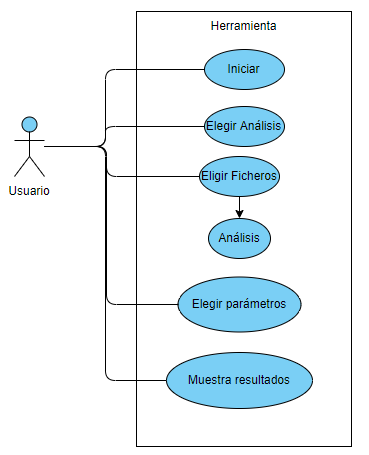
\includegraphics[width=10cm, height=8cm]{Uso}
\caption{Diagrama de casos de uso}
\end{figure}


\include{./tex/C_Diseño}
\apendice{Documentación técnica de programación}



\section{Introducción}
En esta sección se explicaran los conceptos necesarios para poder ponerse a trabajar con este proyecto:\\

Lo primero antes de nada seria descargarse la herramienta desde aquí:\\

Se tiene que descargar desde aquí: \\

\url{https://github.com/Guillecal/TFG-Herramienta_para_medir_la_eficiencia_de_codigo_python/tree/master/Prueba%20TFG\\}



\section{Estructura de directorios}

Los archivos necesarios están metidos en la carpeta Pruebas TFG, dentro de esta esta el archivo principal Vent.py que hace de controlador y vista, y este llama al interprete que  se encuentra dentro de la carpeta byterun. Dentro de esta nos interesa el archivo pyvm2.py que es donde se realizo el upgrade, ademas de ser la partemas importante del interprete.\\

\section{Manual del programador}
Se empezara preparando el entorno de trabajo para trabajar con el proyecto:\\

\subsection{Python}
Para el desarrollo de la herramienta se utilizó la versión de Python 2.7.16, es recomendable descargar esta versión para evitar algún tipo de incoherencia.\\

Link de descarga: \url{https://github.com/Guillecal/TFG-Herramienta_para_medir_la_eficiencia_de_codigo_python/tree/master/Prueba%20TFG\\}

Seguido a esto es necesario instalar las bibliotecas utilizadas dentro del programa. Por ello es necesario comprobar si se tiene instalado primero el sistema de gestión pip, el cual es esencial para poder instalar las bibliotecas faltantes.
Para este proyecto se utilizó la versión 19.1.1, pero en este caso la versión no debería afectar, hay que descargar el contenido que se encuentra en la siguiente dirección, guardar como get-pip.py:\\

Link Descarga: \url{https://bootstrap.pypa.io/get-pip.py}

Despues de de esto en el símbolo de sistemas hay que ejecutar el comando: python get-pip.py\\

Cuando ya se tiene pip instalado ya solo sería meter os siguientes comandos por el símbolo de sistema:\\
pip install matplotlib\\
pip install python-tk\\


\subsection{IDE}
Como entorno de desarrollo se podría se puede utilizar el IDE de Python, pero para el desarrollo de la herramienta se ha utilizado Spyder. \\

Link descaga: \url{https://www.spyder-ide.org}/\\

Una vez descargado e instalado este IDE ya viene listo para empezar poder trabajar, pero en caso de que se requiera, se puden cambiar algunas configuraciones según el gusto de cada uno desde las pestañas Ver y Herramientas.\\

\imagen{Spyder}{Así luce la ventana de Spyder}

Esta es una recomendación, si se está acostumbrado utilizar otro tipo de IDE que sirva para el lenguaje Python no habría ningún problema.\\

\subsection{Github Desktop}

Esta es la herramienta utilizada para gestionar mejor el repositorio donde se encuentra el trabajo
Se puede descargas desde aquí: 

Link: \url{https://desktop.github.com/}\\

Una vez descargado e instalado, la primera vez que lo ejecutamos, podemos clonar desde aquí el proyecto desde el repositorio

\section{Compilación, instalación y ejecución del proyecto}
No se puede compilar al ser Python el lenguaje del código, ya que este es un lenguaje interpretado. Tampoco es necesaria una instalación, por cual lo único que queda por hacer es ejecutar el código.
Hay dos maneras de hacer esto:\\

A través de la línea de comandos\\
A través de un archivo ejecutable\\

\subsection{Linea de comandos}
Esta forma es muy sencilla. Simplemente hay abrir el Símbolo de sistema(Línea de comandos) y navegar hasta el directorio donde se encuentra el archivo Vent.py, esto se puede hacer fácilmente con el comando CD para cambiar de directorio y dir para mostrar los que contiene el directorio actual.\\
Una vez encontrado el directorio simplemente hay que ejecutar el comando: Python Vent.py\\

\subsection{Archivo ejecutable}
Simplemente seria clicar en el archivo .exe que se encuentra dentro de la carpeta dist.\\

Pero para crear este archivo es necesario previamente haber configurado un fichero llamado setup.py que se tiene que encontrar en el mismo directorio que el archivo que se quiere hacer ejecutable, en nuestro caso es dentro de la carpeta prueba TFG. Setup.py se ha configurado de la siguiente manera: \\

\imagen{Setup}{Configuración del fichero setup.py}

Una vez configurado hay que dirigirse al directorio donde se encuentran desde el símbolo de sistema y ejecutar el comando "setup.py py2exe". Con esto deberia generarse una carpeta llamada "dist" y dentro de este se encontrara el ejecutable\\

Como advertencia hay que commentar que podría ser necesario la descarga de un archivo .dll si no se tienen dentro de los archivos de python. 


\section{Pruebas del sistema}
Haré vídeos cuando acabe los cambios en el código.
\apendice{Documentación de usuario}

\section{Introducción}
En esta sección se explica lo necesario para comprender como hacer el funcionamiento de la herramienta a través de unos pasos.
\section{Requisitos de usuarios}
Antes de nada hay que señalar una serie de requisitos previos para que se pueda ejecutar la herramienta:

\begin{enumerate}
	\item Tener un ordenador con una version de Python 2.7 o posterior. junto con las librerías:.
	\item Tener algún tipo de aplicación capaz de crear, leer y escribir archivos deformado .csv (Recomendando MMicrosoft Excel o Apache OpenOffice Calc en su defecto)
	\item Tener disponible algún tipo de  archivo .py para analizar.
\end{enumerate}


No son unos requisitos muy exigentes y una vez cumplidos ya se podría proceder con la instalación sin problemas.

\section{Instalación}
Realmente la herramienta no requiere de ningún tipo de instalación. Simplemente habría que descargar el proyecto del siguiente enlace:\\

\url{https://github.com/Guillecal/TFG-Herramienta_para_medir_la_eficiencia_de_codigo_python}\\

Se descargara un archivo.zip, cuyo contenido hay que extraerlo. Se puede hacer en el directorio que se quiera y una vez hecho simplemente habría que ejecutar el fichero con formato .exe.\\

Pero antes de esto hay que asegurarse de tener algún tipo de fichero.csv en la carpeta Prueba TFG dentro del proyecto, ya que si no, la  herramienta no funcionara como es debido. En principio debería haber algún archivo. csv en el proyecto descargado desde la dirección anterior, pero por si acaso es mejor hacer esta revisión.

\section{Manual del usuario}

Una vez preparados los ficheros y los requisitos previos como esta herramienta no requiere de ningún tipo de configuración posterior, para poder iniciar de forma fácil la herramienta, hay creado un ejecutable que simplemente hay que clicar para iniciar. Cabe destacar que la interfaz de esta herramienta tiene todos los textos en inglés, a pesar de esto en este manual nos referiremos a las distintas opciones en su traducción al español.\\

Una vez este iniciado, muestra una interfaz bastante simple, que nos da a elegir entre tres opciones, Análisis individual, Análisis Múltiple o salir, aquí dependiendo del tipo de uso que se quiera hacer la herramienta, se elegirá uno u otro.\\

\begin{figure}[H]
\centering
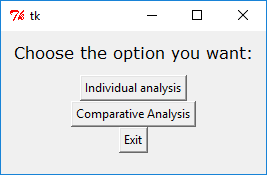
\includegraphics[width=6cm, height=4cm]{VentanaPrincipal}
\caption{Vista de la ventana principal}
\end{figure}

En el caso de querer ver el porcentaje de eficiencia que proporciona cada tipo de operación de un fichero, el análisis individual es la opción adecuada.
Por otra parte si lo que se quiere es hacer una comparación de eficiencia entre ficheros, el análisis Múltiple es el que debes pulsar.


\subsection{Análisis individual}

Si pulsamos el análisis individual, lo primero que nos saldrá será una ventana con dos botones, buscar fichero y volver a la ventana principal.\\
\begin{figure}[H]
\centering
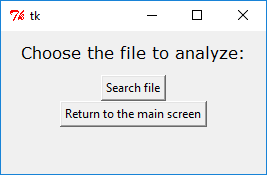
\includegraphics[width=6cm, height=4cm]{VentanaIntermedia}
\caption{Vista de la ventana principal}
\end{figure}
El primero de estos nos permite buscar el fichero que deseamos analizar a través de un explorador de archivos, el archivo seleccionado debe tener un formato.py, ya que si no nos saldrá un mensaje de error indicando que es un tipo de formato no válido.\\
\begin{figure}[H]
\centering
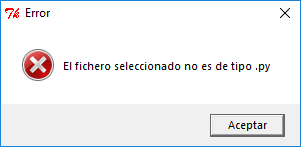
\includegraphics[width=5cm, height=3cm]{Error}
\caption{Mensaje de error}
\end{figure}
Algo parecido aparecerá si no elegimos ningún fichero, como advertencia saldrá  también un mensaje\\
\begin{figure}[H]
\centering
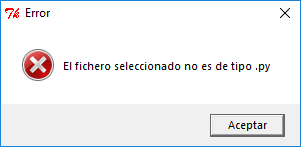
\includegraphics[width=5cm, height=3cm]{Error}
\caption{Mensaje de advertencia}
\end{figure}
Si por el contrario pulsamos el botón de volver a la ventana principal, esto hará que aparezca de nuevo la ventana que se mostró al principio.\\

Una vez seleccionado el archivo .py aparecerá un nuevo botón en el que pondrá analizar fichero. A veces puede que tarde un poco en mostrar el fichero, porque internamente la herramienta tiene que hacer una serie de cálculos.\\
\begin{figure}[H]
\centering
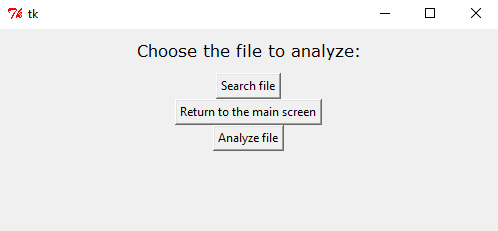
\includegraphics[width=6cm, height=4cm]{VentanaIntermedia2}
\caption{Aparición del botón tras la elección de un archivo .py}
\end{figure}
Si pulsamos ese botón, nos mostrará la ventana de análisis. En esta ventana se muestran los resultados del análisis hecho al fichero que ha sido elegido en la ventana previa. Cuenta con una serie de opciones que hará variar los resultados que serán mostrados.\\

Echando un vistazo de arriba abajo nos encontramos con las siguientes opciones:\\

\begin{enumerate}
	\item Primero al igual que en la ventana anterior a esta, nos encontramos con un botón que nos deja volver a la ventana inicial. Por si queremos realizar algún tipo de análisis más.\\

	\item Despues hay un boton que nos lleva a otra ventana donde se pueden ver unos checkboxes que representan los diferentes tipos de operaciones encontrados en el análisis del fichero seleccionado, que por defecto al principio saldrán todos marcados. Esto indica que operaciones van a ser mostradas en la gráfica de los resultados, si hay algún tipo de operación que no queramos que salga tan solo tendríamos que clicar en el checkbox de la operación para quitarle la marca. Cuando queden marcadas aquellas operaciones que deseemos hay un boton para volver a la vista anterior en la parte de abajo.\\

\begin{figure}[H]
\centering
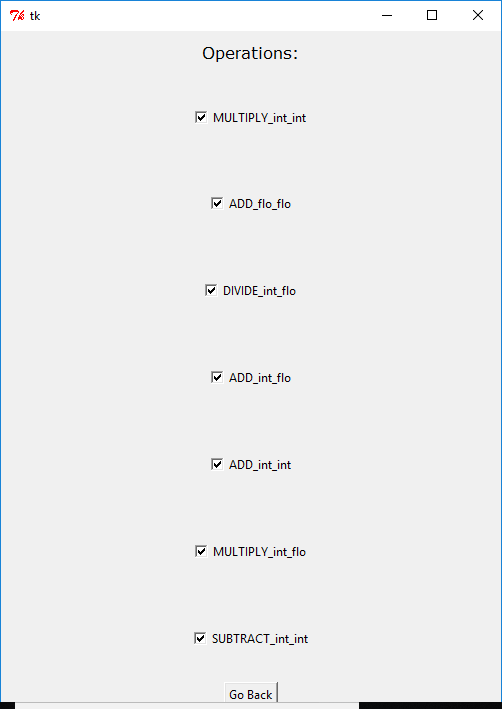
\includegraphics[width=6cm, height=7cm]{Operaciones}
\caption{Ventana donde elegir operaciones}
\end{figure}

	\item Seguido a esto hay una Listbox que deja elegir el procesador con el que se quiere ponderar a las operaciones. En esta lista se muestran los procesadores que tengamos disponibles en la carpeta Prueba TFG. Así que si queremos que aparezcan mas tipos de procesadores tan solo habría que crear más procesadores teóricos ahí.\\

(Se recomienda copiar un procesador ya creado y tan solo tener que cambiar los valores según se desee)\\

\begin{figure}[H]
\centering
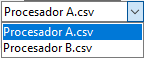
\includegraphics[width=4cm, height=2cm]{ListBox}
\caption{Ejemplo de la Listbox de procesadores}
\end{figure}

	\item Una vez configurados todos estos valores anteriores, habría que pulsar el botón de abajo Mostrar resultados, y tras esto saldría la gráfica resultante.\\
\begin{figure}[H]
\centering
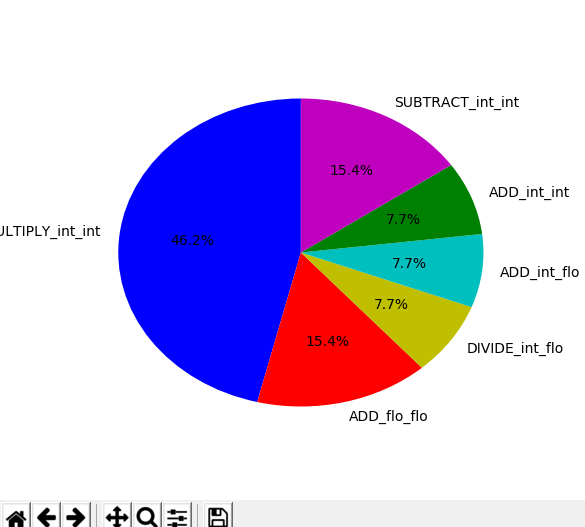
\includegraphics[width=8cm, height=7cm]{Grafica2}
\caption{Ejemplo gráfica resultante análisis individual}
\end{figure}
	\item Hay que tener en cuenta que la configuración puede ser cambiada aunque ya se haya mostrado una gráfica y si se vuelve a pulsar el botón mostrar resultados, vuelve a recargar la gráfica con la nueva configuración que haya sido elegida.\\

\begin{figure}[H]
\centering
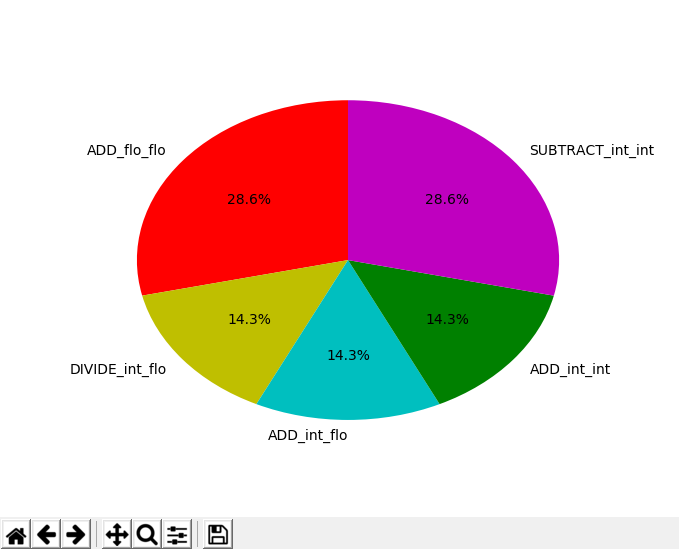
\includegraphics[width=8cm, height=7cm]{Grafica3}
\caption{Ejemplo gráfica resultante recalculada}
\end{figure}

\end{enumerate}

En este caso se ha quitado la marca de la multiplicación de enteros y vemos como este desaparece de la gráfica. Esto mismo se podría hacer también con la listbox de los procesadores.

La gráfica muestra los porcentajes de ciclos de reloj que consume cada tipo de operación. Cada uno diferenciado por un color e indicado con el nombre de la operación y el nombre del tipo de los dos operadores.

Como se puede ver en la última imagen en la parte de abajo hay una serie de botones que nos permiten hacer un par de interacciones con el gráfico como por ejemplo ampliar la zona deseada o poder guardarla.

\subsection{Análisis Múltiple}
Pulsando el botón de análisis Múltiple, Muestra una ventana con dos tipos de opciones, Buscar ficheros y volver a la ventana inicial. Esta ventana es prácticamente idéntica a la primera que sale en el análisis individual (Figura B2). Pero la diferencia que hay en esta se trata del botón buscar ficheros, con el cual sale un explorador de archivos pero con el que hay que seleccionar mas de un fichero. Al igual que en el análisis individual solo se pueden elegir ficheros con formato .py pero además no se puede elegir solo 1 fichero, ya que se hace alguna de estas dos cosas saldrá un mensaje de error.\\

\begin{figure}[H]
\centering
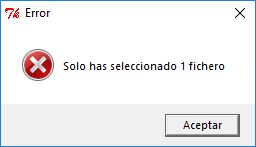
\includegraphics[width=5cm, height=3cm]{Error2}
\caption{Mensaje de error por elegir solo un fichero}
\end{figure}

Una vez seleccionado el fichero saldrá el botón de Analizar, y este nos pasará a la ventana de análisis.\\
Lo primero que vemos en la ventana de análisis es el botón de volver al menú principal en caso de que deseemos hacer el otro tipo de análisis o el mismo con otros ficheros.\\

Seguido hay una listbox que para indicar el procesador teórico con el que se desea ponderar  las operaciones sacadas por el intérprete.\\
Seguido a esto hay un botón que nos lleva a otra ventana donde hay una serie de checkboxes, pero a diferencia del análisis individual, aquí muestra todas las diferentes operaciones que aparecen en todos los ficheros. Así que puede haber operaciones del checkbox que se encuentren solo en un fichero.\\
Una vez elegidos los parámetros está el botón mostrar resultados que nos muestra la gráfica resultante, según los parámetros establecidos. La gráfica se  puede volver a recalcular sin salirse de la ventana volviendo a  pulsar el botón de mostrar resultados y mostrara la gráfica según como estén los parámetros.\\

La gráfica muestra los ciclos de reloj totales que suman todas las operaciones en cada uno de los ficheros seleccionados, a través de una gráfica de barras, si se han seleccionado menos de 10 ficheros y en caso contrario, a través de un gráfico de puntos. Los nombres de los ficheros en la gráfica son sustituidos por letras en orden alfabético. Y como se ha indicado antes para ver el nombre de cada uno hay que buscar en la celda de texto que fichero está asociado a cada nombre.\\

\begin{figure}[H]
\centering
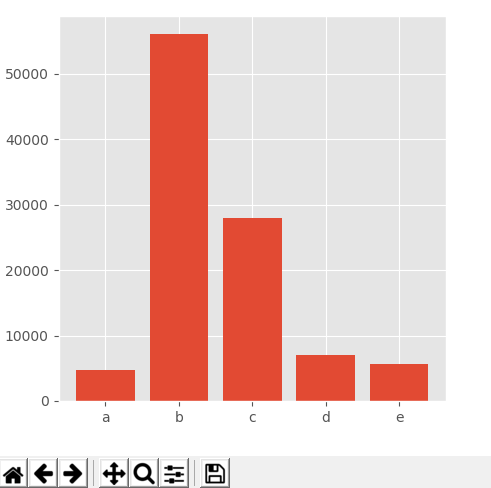
\includegraphics[width=9cm, height=10cm]{Grafica5}
\caption{Gráfico de barras resultante}
\end{figure}

\begin{figure}[H]
\centering
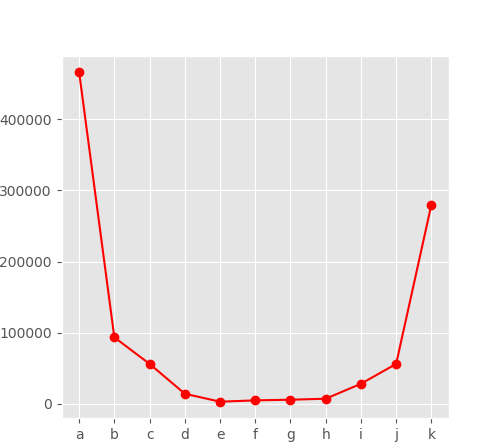
\includegraphics[width=9cm, height=10cm]{Grafica6}
\caption{Gráfico de puntos resultante}
\end{figure}






\bibliographystyle{plain}
\bibliography{bibliografiaAnexos}

\end{document}
